\section{Evaluation}
\label{sec:eval}
\iffalse
Evaluation (don't forget to interpret your data)
\fi
In this section, we present an example which explores the root permission of Docker process. We first describe the experiment set-up, and then discuss the attack example results.

\subsection{Hadoop setup with Docker configuration}
\begin{table}[ht]
\begin{tabular}{|l|l|}
\hline 
Name & Version \\ 
\hline 
CPU & 4 cores, Intel(R) Core(TM) i7-3770 \\
& CPU @ 3.4GHz \\ 
\hline 
Memory & 16 GB \\ 
\hline 
Operating System & Ubuntu 14.04.2 LTS \\ 
\hline 
Hadoop & Version 2.6.0, per \\ 
\hline 
Docker & Version 1.5.0, build a8a31ef \\ 
\hline 
Disk & Usage less than 90\% \\ 
\hline 
\end{tabular}
\label{experiment}
\end{table}

\begin{figure}[h]
  \centering
  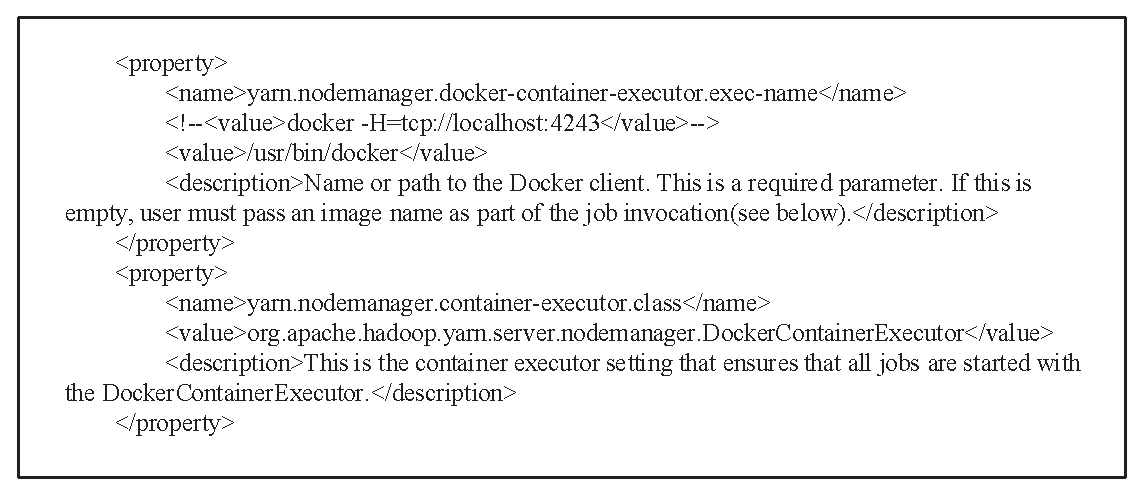
\includegraphics[width=3.3in]{figs/code.eps}
  \caption{Docker container configurations in yarn-site.xml}
  \label{fig:CodeOverview}
\end{figure}
\begin{figure}[h]
  \centering
  \includegraphics[width=3.2in]{figs/command.eps}
  \caption{Hadoop command to run Teragen with the Docker container}
  \label{fig:Commandoverview}
\end{figure}
The experiment platform is shown in the table \ref{experiment}. Hadoop has requirements of minimum resources(e.g., the free disk space should be larger than 10\% of total disk space). The steps for the experiment are described as follows:
\begin{itemize}
\item {Install Hadoop in Pseudo-Distributed mode.}
\item {Install Docker and download Docker image for Hadoop the Docker container.}
\item {Add the properties to yarn-site.xml shown in Figure \ref{fig:CodeOverview}.}
\item {Change the permission of docker command with ``sudo chmod u+s /usr/bin/docker” in order for Hadoop to use Docker container.}
\item {Go to the directory of Hadoop installation, and start Hadoop with ``sbin/start-dfs.sh” and ``sbin/start-yarn.sh”.}
\item {Run ``jps” command and check the running processes: NameNode, SecondaryNameNode, DataNode, ResourceManager, and NodeManager.}
\item {Run Hadoop example program Teragen to generate 1000 bytes of data with the command shown in Figure \ref{fig:Commandoverview} in order to test the usage of the Docker container in Hadoop.}
\item {Run ``docker ps” command after the job is launched and finds that there are 3 containers that are launched to run the Teragen program. The 3 containers terminate after the job is finished.}
\end{itemize}

\subsection{Example attack}
\begin{figure}[t]
  \centering
  \includegraphics[width=3.2in]{figs/attack.png}
  \caption{Attack experiment}
  \label{fig:AttackOverview}
\end{figure}
Figure \ref{fig:AttackOverview} shows the results of launching an attack toward the Hadoop MapReduce job. This attack explores the security vulnerabilities introduced by Docker. Running containers with Docker implies running the Docker daemon which requires root privileges~\cite{rootdocker}. Therefore, in order to use the Docker daemon to create the Docker container, the user running Hadoop should have root privileges which can be achieved through changing the Docker daemon permissions with ``setuid". In this way, the Docker command is able to be run by any user. Malicious users which do not have root privileges can use the command ``docker stop containerID” to terminate the Docker containers that are running Map or Reduce tasks. Terminating the tasks unexpected could lead to MapReduce job failures as shown in the Figure.

